\chapter{Inflation, Structure, and the Fate of Initial Conditions}

These notes follow Leonard Susskind's eighth lecture on cosmology, with the order of the argument and the strongest surviving board evidence kept close to the way the lecture actually unfolds. The classroom record is due to Leonard Susskind, LazyingArt LLC, and Video2Book. The lecture begins with a student's interruption about \(\Omega\), turns that interruption into a discussion of what we really know about the present universe, and then moves toward inflation as the proposed explanation of that knowledge. But the lecture never lets inflation stand as a slogan. At each stage a success creates a new problem: flatness demands inflation, inflation threatens structure, structure forces quantum fluctuations, and the explanatory power of inflation finally becomes an obstacle to recovering what came before it.

\section{Omega, Vacuum Energy, and the Evidence for Flatness}

A student asks what big \(\Omega\) means, and Susskind immediately backs up to the Friedmann equation. There are several omegas in geometry and cosmology; this one is the cosmological bookkeeping device, not the \(\Omega\) that denotes a sphere. The point is to understand how the expansion equation is organized in the late universe.

For the era of interest, well after radiation domination and including the present epoch, the Friedmann equation may be written as
\begin{equation}
H^2=\left(\frac{\dot a}{a}\right)^2=\frac{8\pi G}{3}\,(\rho_0+\rho_m)-\frac{k}{a^2},
\end{equation}
where \(H=\dot a/a\), \(\rho_0\) is the vacuum-energy density, and \(\rho_m\) is the nonrelativistic matter density. Radiation could be added, but in the present universe it is so small that the lecture drops it at once. The important contrast is the way the two surviving energy densities scale:
\begin{equation}
\rho_0=\text{constant},
\qquad
\rho_m=\frac{M}{a^3}.
\end{equation}
Matter dilutes; vacuum energy does not.

At this point the transcript becomes rough, and the algebra on the board is not fully recoverable line by line. What the lecture is clearly doing, however, is dividing the Friedmann equation by \(H^2\) and reading the resulting terms as normalized fractions of the expansion budget. Since the spoken notation wanders among \(\Omega_0\), \(\Omega_{\rm vac}\), and \(\Omega_\Lambda\), we standardize once and for all:
\begin{equation}
\Omega_\Lambda=\frac{8\pi G\,\rho_0}{3H^2},
\qquad
\Omega_m=\frac{8\pi G\,\rho_m}{3H^2},
\qquad
\Omega_k=-\frac{k}{a^2H^2}.
\end{equation}
Then
\begin{equation}
\Omega_\Lambda+\Omega_m+\Omega_k=1.
\end{equation}
In particular, if the universe is flat, \(k=0\), and therefore
\begin{equation}
\Omega_\Lambda+\Omega_m=1.
\end{equation}

That is the cleaned mathematical statement of what Susskind wants to say: \(\Omega\) is the fraction of the expansion equation carried by the various forms of energy. Matter here includes dark matter. If the matter and vacuum terms add to more than one, then \(k>0\) and space is positively curved. If they add to less than one, then \(k<0\) and space is negatively curved. If they add to one, space is flat.

The lecture then turns from notation to evidence, and the order matters. First one measures ordinary matter and dark matter. The latter is not seen directly, but inferred gravitationally from things like stellar orbits in galaxies. Next one measures the Hubble expansion itself. Next one measures the curvature geometrically, by large-scale triangulation. Finally one notices that the universe is not merely expanding, but accelerating. In the lecture's language, the direct evidence for vacuum energy is not \(H\) by itself, but the fact that \(H\) is tending toward a constant, so that
\begin{equation}
a(t)\propto e^{Ht}.
\end{equation}
If \(\dot a/a\) becomes nearly constant, then one is on the exponential branch.

This is the first important beat of the chapter. Flatness is not introduced as a prejudice. It is presented as an empirical fact, checked several ways. Matter plus dark matter, the Hubble expansion, and the geometrical measurement of curvature all point in the same direction: however the universe got that way, it is very nearly flat, to within a few percent.

\section{Why Flatness Is Not Enough: The Need for Structure}

Once the evidence is on the table, Susskind asks the natural next question: why is the universe so flat? His answer is inflation. To say that the universe is flat, in the lecture's deliberately physical language, is to say that it is very big, very smooth, and very homogeneous on scales of billions, really tens of billions, of light years. Inflation is the conjectured early period of exponential expansion that stretches the universe into just such a state.

But now one can overdo a good thing. A perfectly smooth universe stays perfectly smooth. Gravity does not manufacture lumpiness out of exact symmetry. If the universe were exactly homogeneous, there would be no galaxies, no stars, no planets, and no observers to ask what \(\Omega\) means.

Tracing the present universe backward, the lecture places the primordial inhomogeneities at the level of roughly one part in \(10^5\) by the time of transparency:
\begin{equation}
\frac{\delta\rho}{\rho}\sim 10^{-5}.
\end{equation}
The universe was therefore extraordinarily smooth, but not perfectly so. There was a slight wiggliness in the density on many scales.

What happens next is the gravitational instability story. Small overdensities attract matter from nearby regions. Those nearby regions then become more underdense, which makes the original overdensities stand out even more strongly. Self-gravity amplifies the contrast rather than erasing it.

\begin{figure}[t]
\centering
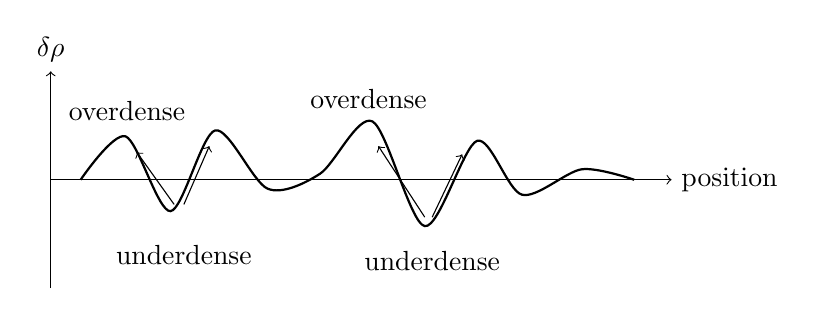
\begin{tikzpicture}[scale=0.95]
\draw[->] (0,-1.45) -- (0,1.45) node[above] {\(\delta\rho\)};
\draw[->] (0,0) -- (8.3,0) node[right] {position};
\draw[thick] plot[smooth] coordinates {
(0.4,0.00) (1.0,0.58) (1.6,-0.42) (2.2,0.66)
(2.9,-0.12) (3.6,0.08) (4.3,0.78) (5.0,-0.62)
(5.7,0.52) (6.3,-0.20) (7.1,0.14) (7.8,0.00)
};
\draw[->] (1.65,-0.33) -- (1.15,0.37);
\draw[->] (1.78,-0.33) -- (2.12,0.45);
\draw[->] (5.00,-0.50) -- (4.38,0.45);
\draw[->] (5.10,-0.50) -- (5.50,0.34);
\node at (1.02,0.92) {overdense};
\node at (4.25,1.08) {overdense};
\node at (1.78,-1.00) {underdense};
\node at (5.10,-1.08) {underdense};
\end{tikzpicture}
\caption{A transcript-backed schematic of the lecture's structure-formation story. Gravity deepens the overdense regions and empties out the underdense regions, so the contrast grows.}
\end{figure}

This is where the lecture draws a sharp contrast with ordinary matter in a room. If we made a small density perturbation in the air around us, pressure and thermalization would erase it. Air returns to equilibrium. Gravity does the opposite. Under self-gravity a little overdensity tends to grow into a bigger one.

The lecture also reminds us that what we directly observe on the sky is not the mass density itself but temperature anisotropy in the cosmic microwave background. Some of that temperature pattern comes from density fluctuations, some from velocity fluctuations, and the mapping is not trivial. Overdense regions tend to look slightly colder because photons lose more energy climbing out of deeper gravitational wells, though Doppler shifts from the motion of the gas are superposed on top of that. The numerical analysis is complicated. The robust conclusion is not: by the time the universe became transparent, there were already fluctuations of order \(10^{-5}\).

\section{Pressure, Matter Domination, and the Onset of Collapse}

At this point a student asks exactly the right question: if gravity amplifies overdensities, why did it not do so much earlier? Susskind's answer is immediate: pressure. The lecture returns to the equation-of-state relation
\begin{equation}
p=w\rho,
\end{equation}
and asks us to remember the values
\begin{equation}
w_{\rm rad}=\frac13,
\qquad
w_m=0,
\qquad
w_{\rm vac}=-1.
\end{equation}

The qualitative meaning is what matters. Radiation has positive pressure, and positive pressure homogenizes. It pushes disturbances out and tends to smooth the medium. That is why ordinary gases do not spontaneously collapse into lumps. Matter, by contrast, is effectively pressureless in the cosmological approximation. If one imagined a medium with \(p=0\) and no gravity, any inhomogeneity would simply sit there, frozen in. But once gravity is present, the absence of pressure support means there is nothing to prevent an overdensity from pulling matter inward.

So there is a competition:
\begin{equation}
\text{gravity} \qquad \text{versus} \qquad \text{pressure}.
\end{equation}
During the radiation-dominated era the pressure was so large that it prevented gravity from doing its work. Later, when radiation became dynamically unimportant, gravity won and the lumps began to contract.

Dark matter enters at precisely this stage. The lecture is careful about the order. First the dark matter fluctuations begin to make large halos. The pressure is small, so those fluctuations can grow. Ordinary baryonic matter then falls into the dark halos, but baryons do require true dissipative processes if they are to settle toward the centers and make luminous galaxies. Dark matter does not dissipate in that way, so it remains as the extended halo.

There is also a timing subtlety that the lecture wants us to keep in mind. The matter-radiation crossover is not exactly the same event as transparency or recombination. Dark matter began to contract a little earlier, perhaps by a factor of ten in time, before the universe became transparent. That is why we do not directly see the beginning of the contraction in the microwave background. We see it only after the fact.

And here the lecture leaves us with a useful promise. In ordinary mechanics one expects dissipation to matter whenever energy is to be degraded. Susskind says there is also a cosmological kind of dissipation, one tied to expansion itself, and that we will need it later. This is not yet the inflaton story, but it is already the right intuition.

\subsection{Question \& Answer}

\paragraph{Why didn't gravity make galaxies earlier?}

Because earlier on the universe was radiation dominated, and radiation carries positive pressure. With \(p=\rho/3\), the radiation bath resists gravitational clumping and tends to homogenize the medium. Only after matter became more important than radiation did pressure cease to block collapse.

Dark matter could begin this process first. Its pressure was effectively negligible, so its small fluctuations grew into halos before ordinary matter could settle into stars and galaxies. The baryons followed later, and because they can dissipate, they collected nearer the centers of those halos.

\section{The Inflaton and Its Potential}

Only after the flatness problem and the structure problem are both alive does the lecture introduce the mechanism of inflation itself. The basic object is a scalar field \(\phi\). Its energy density has three pieces:
\begin{equation}
\rho_\phi=\frac12\dot\phi^2+\frac12(\nabla\phi)^2+V(\phi).
\end{equation}
The first term is due to time variation, the second to spatial variation, and the third is the potential-energy density.

Susskind motivates this by comparison with more familiar fields. An electromagnetic field has energy from its time dependence and from its spatial gradients. A scalar field has those same two kinds of energy, but in addition it may have a genuine potential \(V(\phi)\). That is not exotic. The Higgs field is the standard example of a scalar field with a nontrivial potential. What is unusual here is the shape of the potential needed for inflation.

At the level of the lecture, the shape is more important than the microscopic origin. The field is supposed to sit at some value of \(\phi\) on a broad, almost flat plateau. This is not a place in space; it is a value of the field. If the field initially varied a bit from place to place, inflation would stretch those wrinkles to such enormous scales that our observable patch would lie deep inside one nearly uniform region. That is why, for the later derivation, we are entitled to treat the field as approximately homogeneous.

\begin{figure}[t]
\centering

\includegraphics[width=0.76\textwidth]{lecture_08_figure_03.png}
\caption{Inflationary potential with plateau and minimum. The lecture uses this blackboard sketch to emphasize the broad plateau, the steep drop, and the low residual minimum.}
\end{figure}

The board sketch is only qualitative, but the qualitative structure is clear enough to preserve. The potential is high and nearly flat over some range, slopes gently downward, then falls sharply, reaches a low minimum, and rises again on the other side.

\begin{figure}[t]
\centering
\begin{tikzpicture}[scale=0.95]
\draw[->] (-0.2,0) -- (7.5,0) node[right] {\(\phi\)};
\draw[->] (0,-0.2) -- (0,4.25) node[above] {\(V(\phi)\)};
\draw[thick] (0.40,3.40)
.. controls (1.30,3.42) and (2.30,3.38) .. (3.00,3.16)
.. controls (3.38,3.02) and (3.68,2.72) .. (3.92,1.76)
.. controls (4.10,0.92) and (4.35,0.32) .. (4.75,0.26)
.. controls (5.05,0.21) and (5.36,0.42) .. (5.70,0.82)
.. controls (6.08,1.28) and (6.55,2.00) .. (7.05,3.02);
\draw[dashed] (0.45,2.10) -- (3.55,2.10);
\end{tikzpicture}
\caption{A qualitative redraw of the potential. The axis labels are note-writer reconstructions from the transcript; the robust content is the plateau, the cliff, the low minimum, and the rising branch.}
\end{figure}

The lecture repeatedly insists that this is a cartoon, not a derived potential. It is contrived in the modest sense that some parameters have to be tuned. But it captures the dynamics we want. The field begins high on the plateau, rolls slowly, then goes over the edge. The minimum is not exactly zero. In Planck units the present vacuum energy is tiny,
\begin{equation}
V_{\rm today}\sim 10^{-123},
\end{equation}
so the minimum must sit at a very small positive value. The plateau during inflation was much higher than this, though still much smaller than the Planck scale.

Now the key physical point: as long as the plateau is flat enough and the field is moving slowly enough, the first two terms in \(\rho_\phi\) are negligible compared with \(V(\phi)\). The field therefore behaves as a vacuum-energy source. The lecture writes this only schematically on the board, so we restore the standard normalization in print:
\begin{equation}
H^2\simeq \frac{8\pi G}{3}\,V(\phi),
\qquad
a(t)\propto e^{Ht},
\end{equation}
with the understanding that the lecture itself only insists on the proportionality
\begin{equation}
H\propto \sqrt{V(\phi)}.
\end{equation}
If \(V(\phi)\) were perfectly flat and \(\phi\) just sat still, this would be exactly vacuum-energy expansion.

The lecture's picture is then deliberately stark. All of cosmology, in this cartoon, is the story of a field rolling from high up on a potential toward a low minimum. Almost everything we can observe happened after the field went over the cliff. Going over the edge is where the large vacuum-like energy of the plateau was converted into more familiar energy: radiation, ordinary matter, dark matter, and a very small leftover vacuum energy.

\section{Slow Roll, Reheating, and Hubble Friction}

At this point the lecture raises the next obstacle. If the field falls off the edge, why should it not simply slosh forever? Why should it not overshoot, swing back, and perhaps even climb again? In ordinary mechanics one would ask where the dissipation came from. Susskind's answer is that cosmology provides its own dissipation. It is not genuine microscopic friction, but it behaves mathematically like friction.

To see it, we simplify exactly as the lecture does. We neglect the spatial gradients of the field, because inflation has stretched them out. We then treat \(\phi(t)\) as an effective homogeneous degree of freedom. The top line of the board is cropped, so the Lagrangian must be regularized cautiously. The cleaned homogeneous form is
\begin{equation}
L_{\rm eff}=a^3(t)\left[\frac12\dot\phi^2-V(\phi)\right].
\end{equation}
The factor \(a^3\) is essential. The field terms are energy densities, and to get the effective Lagrangian for the homogeneous mode we multiply by the physical volume.

\begin{figure}[t]
\centering

\includegraphics[width=0.76\textwidth]{lecture_08_figure_05.png}
\caption{Scalar-field equation with Hubble friction. The board shows the Euler--Lagrange form and the final damped equation; the top Lagrangian line is only partial and is regularized in the text.}
\end{figure}

Now we work through the derivation in the same spirit as the lecture. First,
\begin{equation}
\frac{\partial L_{\rm eff}}{\partial\dot\phi}=a^3\dot\phi.
\end{equation}
The Euler--Lagrange equation then gives
\begin{equation}
\frac{d}{dt}\left(a^3\dot\phi\right)=\frac{\partial L_{\rm eff}}{\partial\phi}
=-a^3\frac{\partial V}{\partial\phi}.
\end{equation}
This is one of the secure board equations. Expanding the time derivative,
\begin{align}
\frac{d}{dt}\left(a^3\dot\phi\right)
&=a^3\ddot\phi+3a^2\dot a\,\dot\phi.
\end{align}
Dividing by \(a^3\) and writing \(\dot a/a=H\), we obtain
\begin{equation}
\ddot\phi+3H\dot\phi=-\frac{\partial V}{\partial\phi}.
\end{equation}
The lecture explicitly corrects the sign at the board: the force is minus the derivative of the potential. That corrected sign is the one shown here.

This is the promised cosmological dissipation. The term \(3H\dot\phi\) is what Susskind calls Hubble friction. It is not true friction. It came from differentiating the factor \(a^3(t)\). But dynamically it behaves like the viscous drag on an object moving through a fluid. The lecture's analogy is a rock falling through water. There is a force term, an acceleration term, and a term linear in the velocity that rapidly brings the motion to terminal speed.

That is the slow-roll idea in the language actually used in the lecture. If the slope is shallow, the terminal velocity is small. If the terminal velocity is small, the field moves only slowly across the plateau. During that long slow slide the potential energy remains almost constant, so the expansion remains almost exponential.

The field does eventually reach the cliff and then the minimum. Once it is near the minimum it oscillates, and those oscillations are just the quanta of the inflaton field. If those quanta are unstable, they decay into photons, electrons, positrons, and other ordinary particles. That is the lecture's reheating picture. The vacuum-like energy on the plateau is converted into the hot matter and radiation content of the post-inflationary universe.

\subsection{Question \& Answer}

\paragraph{Why doesn't the inflaton oscillate forever?}

Because the expansion of the universe itself damps the motion. The term \(3H\dot\phi\) continually degrades the coherent motion of the field, in much the same way that viscosity degrades the motion of a particle in a fluid. Then, once the field is oscillating near the minimum, those oscillations are the inflaton quanta, and if the quanta are unstable they decay into more familiar forms of matter and radiation. The sloshing is not protected; it is redshifted and then converted.

\section{Quantum Fluctuations, Horizon Exit, and Scale Invariance}

Now the lecture turns the knife once more. If inflation expands the universe by many orders of magnitude, should it not iron out every last irregularity? On the face of it, inflation seems almost too good. It explains flatness and homogeneity, but threatens to erase the very seeds that galaxies need. Susskind's answer is that the surviving irregularities are not leftover classical wrinkles. They are generated anew by quantum mechanics.

The lecture first asks us to forget expansion for a moment. Take a field that has already been ironed nearly uniform. Why should it still fluctuate? Because of the uncertainty principle. One cannot lock both \(\phi\) and its velocity into exact values. The ground state of the field is therefore not dead still. It is agitated by zero-point motion, just as the ground state of a harmonic oscillator carries zero-point energy.

Why do we not ordinarily notice that agitation? Because most of the fluctuations are short wavelength, and short wavelengths oscillate rapidly. We average over them. In ordinary circumstances the field fluctuates too fast for those fluctuations to show up macroscopically.

Cosmology changes the story because the universe expands. We use a comoving coordinate \(x\), which labels positions but is not itself a physical distance. The physical separation between two fixed comoving positions is
\begin{equation}
\lambda_{\rm phys}=a(t)\,\Delta x.
\end{equation}
During inflation the scale factor grows nearly exponentially, while the physical Hubble scale is approximately fixed:
\begin{equation}
d_H=\frac{c}{H}\simeq H^{-1}
\qquad (c=1).
\end{equation}
Therefore the comoving horizon shrinks:
\begin{equation}
d_{H,\mathrm{coord}}=\frac{1}{aH}.
\end{equation}

\begin{figure}[t]
\centering
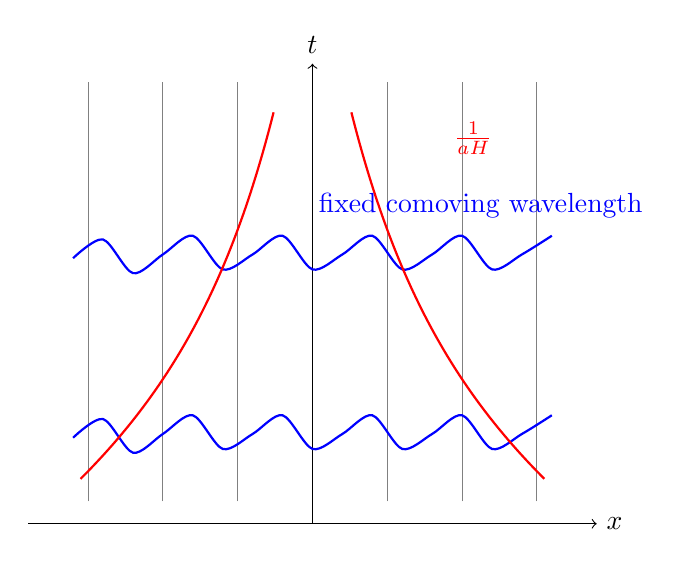
\begin{tikzpicture}[scale=0.95]
\draw[->] (-3.8,0) -- (3.8,0) node[right] {\(x\)};
\draw[->] (0,0) -- (0,6.15) node[above] {\(t\)};
\foreach \x in {-3,-2,-1,1,2,3}
  \draw[gray] (\x,0.30) -- (\x,5.90);
\draw[thick,blue] plot[smooth] coordinates {
(-3.2,1.15) (-2.8,1.40) (-2.4,0.95) (-2.0,1.20) (-1.6,1.45)
(-1.2,1.00) (-0.8,1.20) (-0.4,1.45) (0.0,1.00) (0.4,1.20)
(0.8,1.45) (1.2,1.00) (1.6,1.20) (2.0,1.45) (2.4,1.00)
(2.8,1.20) (3.2,1.45)
};
\draw[thick,blue] plot[smooth] coordinates {
(-3.2,3.55) (-2.8,3.80) (-2.4,3.35) (-2.0,3.60) (-1.6,3.85)
(-1.2,3.40) (-0.8,3.60) (-0.4,3.85) (0.0,3.40) (0.4,3.60)
(0.8,3.85) (1.2,3.40) (1.6,3.60) (2.0,3.85) (2.4,3.40)
(2.8,3.60) (3.2,3.85)
};
\draw[red,thick] (-3.1,0.60) .. controls (-1.9,1.80) and (-1.1,3.20) .. (-0.52,5.50);
\draw[red,thick] (3.1,0.60) .. controls (1.9,1.80) and (1.1,3.20) .. (0.52,5.50);
\node[blue] at (2.25,4.25) {fixed comoving wavelength};
\node[red] at (2.15,5.15) {\(\frac{1}{aH}\)};
\end{tikzpicture}
\caption{A comoving spacetime sketch for mode freezing. The mode keeps roughly the same coordinate wavelength, while the comoving horizon shrinks. Once the mode lies outside the horizon, it freezes.}
\end{figure}

The lecture explains the freezing with a rope analogy. A wave oscillates because each bit of rope is pulled by neighboring bits. But if the wavelength becomes as large as the horizon, the relevant neighbors lie beyond causal contact. They cannot communicate their pull. The restoring force disappears. Mathematically the result is that once a mode becomes longer than the horizon, it ceases to oscillate:
\begin{equation}
\lambda_{\rm phys}\gtrsim H^{-1}
\qquad \Longrightarrow \qquad
\text{freeze-out}.
\end{equation}

That happens mode by mode. Longer wavelengths freeze first, shorter wavelengths later, but in an exponentially expanding universe every mode is eventually stretched beyond the horizon. The fluctuations do not vanish. They freeze into classical-looking variations of the field.

This is also where the lecture insists on something subtle and important. It does not matter how long inflation lasts. One might think that enough inflation would wash out everything. But as time goes on, new vacuum fluctuations are continuously generated on short scales, then stretched, then frozen. So the old fluctuations are stretched away, but new ones keep coming in. At a fixed point in space the field undergoes a random walk as one frozen mode after another is added with random phase. At different points in space the random walk is different. That is what builds a statistical pattern of large-scale variation.

The lecture's phrase for the resulting distribution is a scale-invariant spectrum. The exact statement is only approximate, and the lecture does not derive a closed formula for it. The physical claim is that the same freezing process repeats on successive logarithmic scales, so the amplitude comes out roughly the same from one wavelength band to the next.

There is one more step. During inflation there is a temporary, small horizon associated with the vacuum energy on the plateau. After the field falls off the cliff, the horizon grows again. Modes that had been stretched outside this temporary horizon eventually come back in. In the lecture's language they go out of the horizon and later re-enter the horizon. By that time they have been stretched to macroscopic scales, so when they start to slosh again they do so as huge, slowly varying structures.

\subsection{Question \& Answer}

\paragraph{If inflation smooths everything out, why aren't the galaxy seeds erased?}

Because inflation smooths away preexisting classical irregularities, but it does not eliminate quantum zero-point fluctuations. Expansion continually stretches those fluctuations beyond the horizon, where they freeze into real field variations. Inflation therefore removes the old roughness and generates a new one. The galaxy seeds are not leftover dirt from before inflation; they are frozen quantum fluctuations produced during inflation itself.

\section{What Inflation Predicts, What It Hides, and Why Fine-Tuning Returns}

Once those frozen variations exist on the inflaton field, the lecture asks what happens when the field finally reaches the cliff. Here the fluctuations are not magnified in spatial size; inflation has already done that. What is magnified now is their amplitude as density contrasts.

Susskind's way of seeing it is to imagine nearby regions with slightly different values of \(\phi\). Regions a little farther to the right are a little farther downhill and therefore reach the cliff first. Suppose, for simplicity, that when a region falls off the cliff its vacuum energy is converted into radiation. That radiation dilutes with expansion:
\begin{equation}
\rho_r\propto a^{-4}.
\end{equation}
A neighboring region still on the plateau remains vacuum dominated, and vacuum energy does not dilute. Therefore the earlier-falling region has already redshifted part of its energy away by the time the later-falling region finally makes the transition.

This is the origin of the final density contrast. A slightly later region emerges denser, simply because it waited longer before converting its energy into a form that dilutes. In a schematic note-writer reconstruction of the spoken argument,
\begin{equation}
\delta t\sim \frac{\delta\phi}{\dot\phi},
\qquad
\frac{\delta\rho}{\rho}\propto H\,\delta t
\sim H\,\frac{\delta\phi}{\dot\phi}.
\end{equation}
The lecture does not present this as a finished formal formula, so it should be read only as a compact summary of the logic. Its content is exactly what Susskind emphasizes verbally: the flatter the potential, the smaller the terminal velocity \(\dot\phi\); the smaller the terminal velocity, the larger the final density variations. Likewise, the higher the plateau, the larger the fluctuations tend to be.

The width of the plateau plays a different role. It mostly controls how long inflation lasts, that is, how many e-foldings occur:
\begin{equation}
N=\ln\!\frac{a_f}{a_i}=\int_{t_i}^{t_f} H\,dt.
\end{equation}
The height affects the size of \(H\); the width and slope determine how long the field stays on the plateau. So the lecture naturally separates two questions: how big are the fluctuations, and how many e-foldings took place?

If the height of the plateau is large enough, another observable can appear: gravitational waves produced during the inflationary era. Their presence would tell us about the overall height of the potential. Their absence already tells us that the scale cannot be too high. The lecture gives only ballpark numbers here and says so explicitly. In Planck units the interesting window is of order
\begin{equation}
10^{-16}\lesssim V \lesssim 10^{-14},
\end{equation}
up to order-of-magnitude uncertainty. Above that range, one would already have seen an excessive gravitational-wave contribution in the microwave background. Below it, there may be no realistic chance of seeing inflationary tensor modes at all.

Susskind then pauses over the units. The explanation is the standard natural-units one. The Compton wavelength of a particle of mass \(m\) is
\begin{equation}
\lambda_C=\frac{\hbar}{mc}.
\end{equation}
If we set \(c=\hbar=1\), then length has units of inverse mass. Energy density is energy per volume, so it has units
\begin{equation}
[\rho]=(\text{mass})^4.
\end{equation}
That is the sense in which \(10^{-14}\), \(10^{-16}\), or \(10^{-123}\) are being quoted.

At this stage the lecture takes a broader view of what inflation has accomplished. Its success is real. It correlates fluctuations on very different wavelength scales using essentially one underlying picture. But exactly because it stretches away earlier irregularities and replaces them with quantum fluctuations generated later, it also makes the pre-inflationary past difficult to recover. The success of inflation is that it washes out what came before. The problem is that the very same washing-out leaves us with little direct access to what came before.

That is why Susskind becomes cautious about the beginning. To say that the universe ``started'' high on the plateau is not to claim that this is the absolute beginning of everything. It only means that this is as far back as the inflationary description can be trusted in the cartoon. If inflation lasted too long, earlier information is erased. If we were extremely lucky and the number of e-foldings were only barely sufficient, perhaps some trace of an earlier stage might survive. But in general inflation tends to wipe out the past.

The lecture then adds a late geometric caveat. We have been using
\begin{equation}
a(t)\propto e^{Ht}
\end{equation}
throughout, and that is correct for the inflationary branch at late times. But exact de Sitter space is more properly described, in a global slicing, by
\begin{equation}
a(t)\propto \cosh(Ht).
\end{equation}
That solution contracts to a minimum size and then re-expands. Whether the contracting branch should be taken literally in cosmology is left as a question mark in the lecture. The point is not to settle it here, only to avoid mistaking the late-time exponential form for the whole exact story.

Finally the lecture returns to fine-tuning and anthropic reasoning. To first approximation the inflationary model has three parameters: the height \(V_0\) of the plateau, its slope, and its width \(\Delta\phi\). The slope is especially important because it controls the terminal velocity and therefore both the fluctuation amplitude and the duration of slow roll. The lecture remarks that many physicists are uneasy if \(\Delta\phi\) becomes larger than the Planck mass, and more strongly that the energy density should not exceed order one in Planck units. Given such rough bounds, the raw fraction of parameter space that yields enough inflation can be small. In the lecture's illustrative estimate, getting roughly \(60\) to \(62\) e-foldings is a few-percent tuning, on the order of \(2\%\).

But then the lecture changes the question. There are two fine-tuning puzzles on the table. One is this mild tuning of the inflationary plateau. The other is the present cosmological constant, of order \(10^{-123}\). The proposed unifying explanation is anthropic: the universe had to allow structure to form.

For a positive cosmological constant, the Newtonian picture is that of a universal repulsion proportional to distance. If the present vacuum energy were only a couple of orders of magnitude larger than observed, it would already prevent the primordial \(10^{-5}\) fluctuations from condensing into galaxies. That is the lecture's retelling of Weinberg's argument: the cosmological constant need not be exactly zero; it only has to be small enough that structure can form.

Negative curvature leads to the same kind of bound. In the Newtonian language reviewed earlier in the course, \(k<0\) corresponds to recession faster than escape velocity. Too much negative curvature means too much outward thrust, and that also prevents galaxies from forming. Inflation dilutes curvature, so one can ask how many e-foldings are required before structure formation becomes possible. The lecture quotes
\begin{equation}
N_{\min}\approx 59.5,
\qquad
N\gtrsim 62
\end{equation}
as the relevant benchmark. Fewer than about \(59.5\) e-foldings would leave too much curvature for galaxies to condense; our existence therefore tells us that the inflationary history lay beyond that threshold.

This changes the meaning of probability. If one asks for the raw volume of parameter space that gives sufficient inflation, the answer may be only a few percent. But if one conditions on being in a universe where galaxies exist and observers can ask the question, then the forbidden part of parameter space is discarded at the outset, and the conditional probability can become large. The lecture does not present that as the end of the matter. It presents it, very deliberately, as the place where the great puzzles, the great confusions, and the great debates now live.

\section{Summary}

The lecture begins with a student's question about \(\Omega\), because inflation is not introduced in a vacuum; it is introduced as the proposed explanation of an observed fact, namely that the universe is almost flat. Flatness then forces the question of structure, because a universe made too smooth could never make galaxies. That leads to the pressure-versus-gravity story, the special role of dark matter, and finally the inflaton: a scalar field on a shallow potential whose vacuum-like energy drives exponential expansion. The field rolls slowly because expansion itself produces Hubble friction. Inflation does not erase all seeds of structure, because quantum fluctuations are continually created, stretched beyond the horizon, and frozen in. Those frozen fluctuations later re-enter and become the density variations from which galaxies grow. The same framework is impressively successful and deeply frustrating: it explains a great deal by washing out initial conditions, and therefore makes the earlier history correspondingly hard to recover.